\section{Dynamia}
\begin{figure}[H]
  \centering
  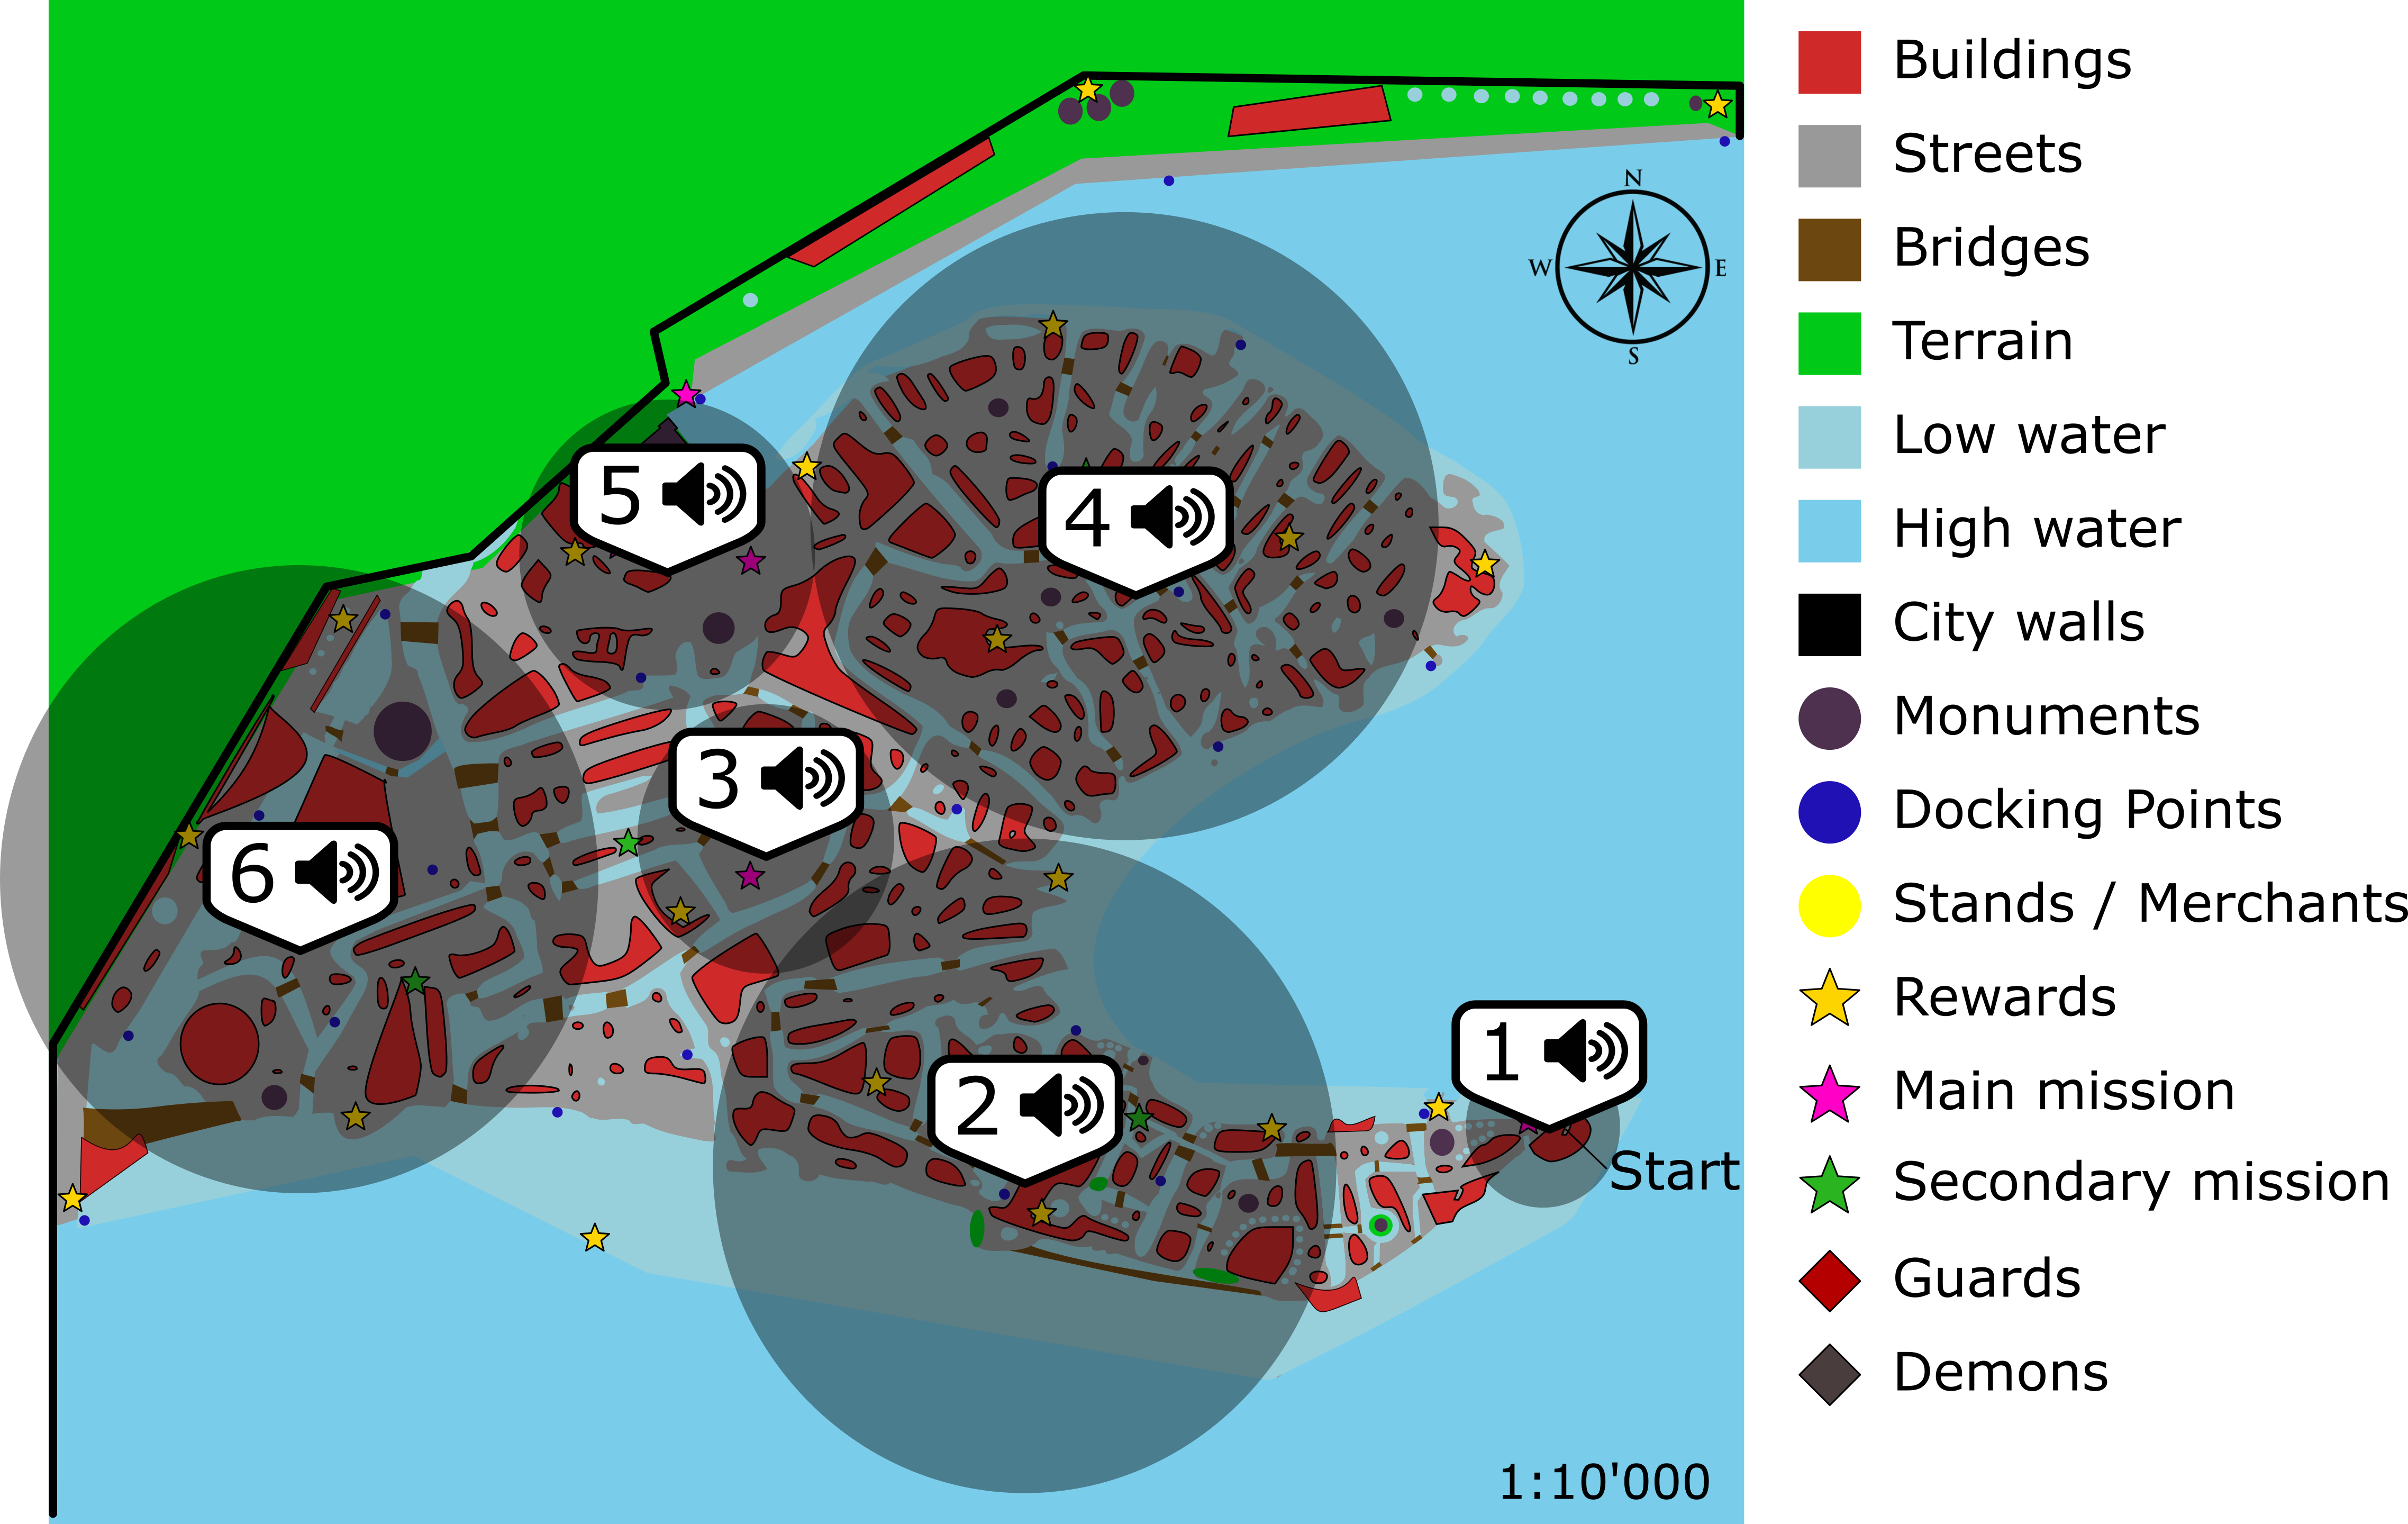
\includegraphics[width=\textwidth]{Images/Maps/dynamiaAudio}
  \caption{Audio points for town center}
\end{figure}

In the whole city there is the sound of the waves, that is more evident when the player is near the sea, and the noises made by the boats, in particular the steam-powered ones.

Sometimes you hear the cry of some seagulls.

\subsection{Harbor area}
The harbor area is the most noisy area of Dynamia. There are the screams of the workers and the noises made by the big boats and the machines.

\subsection{Bystander in a hurry (all areas)}
\textbf{Bystander 1 (running in a hurry)}: Let me through. I'll miss the ferry!

\subsection{Running children (all areas)}
\textbf{Child 1 (happy)}: You can't catch me!

\textbf{Child 2 (happy)}: Wait!

\subsection{Worried merchant (all areas)}
\textbf{Merchant 2 (disappointed)}: My shop is empty. If I don't get supplies soon, I'll be forced to quit.

\subsection{Disappointed fishermen}
\textbf{Old fisherman 1 (disappointed)}: Damn, I need to buy new fishing nets.

\subsection{Fish seller (southern area, ghetto area)}
\textbf{Seller 1 (screaming)}: FISH! FRESH FISH!

\subsection{Disappointed women (southern area, central area)}
\textbf{Woman 1 (disappointed)}: Because of the war there are no more tourists! The inns are all empty!

\textbf{Woman 2 (worried)}: Ssh. A guard may hear you.

\subsection{Boat woman (southern area, harbor area, ghetto area)}
\textbf{Woman 3}: My boat is about to sink. I wonder if I should repair it or buy a new one.

\subsection{Rich women (central area)}
\textbf{Woman 4 (worried)}: I wonder if there will be the Carnival this year.

\textbf{Woman 5 (worried)} I'm worried there will be nothing like that. The mask shops are almost all closed.
